\chapter{环境配置}

本章只是简单介绍一下环境的配置,分为云平台和本地平台两部分。
云平台无需配置,直接使用。
本地部分只是粗略介绍,细节部分可自行搜索获得。
欢迎各位来补充。

\section{云平台}

本模板已经在 \href{https://www.overleaf.com}{OverLeaf}\footnote{一个在线的 \LaTeX 平台} 测试通过。可以直接在 Github 上直接下载为 zip 文件,再导入 OverLeaf 即可。

\section{本地平台}

这部分讲述本地 \LaTeX 环境配置。

本地环境配置主要有三部分,一是 \LaTeX 发行版 TeX Live,二是编辑器 TeXstudio,三是宏包依赖项的安装。

\subsection{TeX Live}

在 \href{https://mirrors.tuna.tsinghua.edu.cn/CTAN/systems/texlive/Images/}{清华镜像} 下载 texlive.iso 文件。
然后进行安装,详细安装教程请自行查阅。

\subsection{TeXstudio}

在 \href{http://texstudio.sourceforge.net/}{官网} 下载安装即可。

中文模板建议使用 XeLaTeX 编译,由于参考文献调用了 biber,需要使用更改 TeXstudio 相应配置,如 \autoref{fig:xelatex-biber} 所示。

\begin{figure}[H]
    \centering
    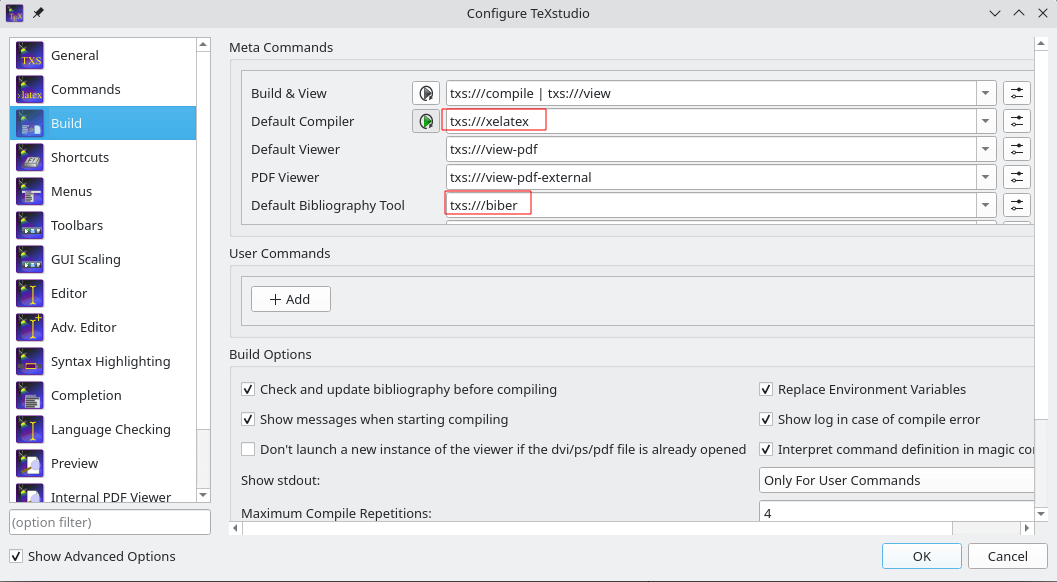
\includegraphics[width=0.8\textwidth]{img/xelatex-biber.png}
    \caption{构建命令选择}
    \label{fig:xelatex-biber}
\end{figure}

同时,代码高亮宏包 minted 需要调用外部命令,进行如 \autoref{fig:xelatex-shell-excape} 所示的设置。

\begin{figure}[H]
    \centering
    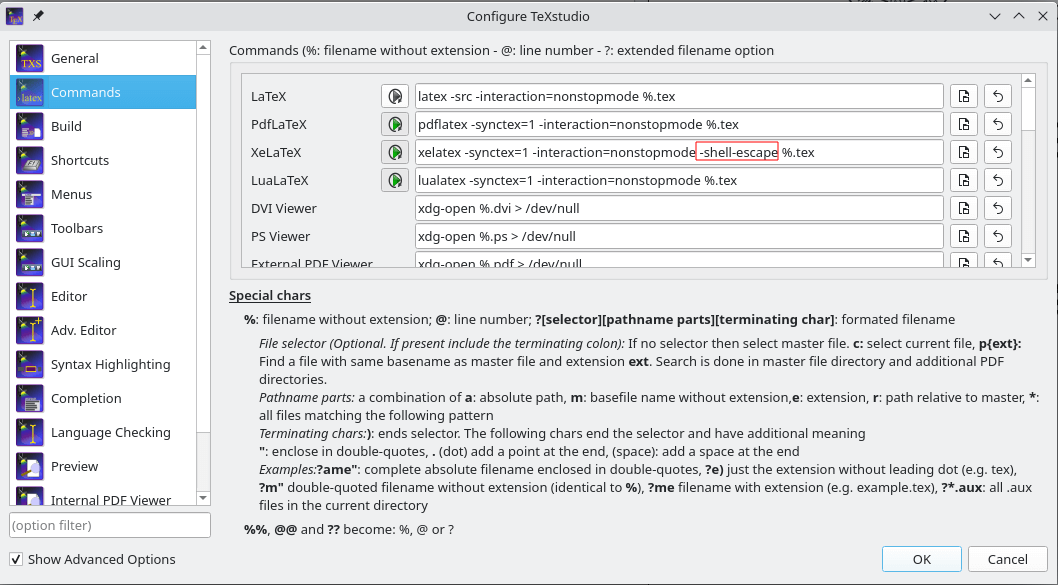
\includegraphics[width=0.8\textwidth]{img/xelatex-shell-escape.png}
    \caption{编译器外部命令设置}
    \label{fig:xelatex-shell-excape}
\end{figure}

\subsection{依赖项}

代码高亮部分使用了 minted 宏包,该宏包依赖 pygmentize(python 库),可以通过如下命令来安装 pygmentize。

\begin{minted}[]{sh}
pip install Pygments
\end{minted}

如果不需要该宏包的话,则在 scutthesis.cls 将 \verb|\|RequirePackage{minted} 以及 tex 中相关使用删除即可。